\section{Numerical Experiments}
\label{sec:experiments}

We evaluate (Nested) WAIT using Microsoft Vidur (simulating NVIDIA A100) \citep{agrawal2024vidur} on synthetic and real datasets \cite{zheng2023lmsys}. Benchmarks: vLLM \citep{kwon2023efficient} and Sarathi \citep{agrawal2023sarathi} (FCFS-based engines).

\subsection{WAIT Algorithm (Known Output Lengths)}
We test two scenarios with Poisson arrivals:
(i) \textbf{Low demand}: \( m=2 \), \( (l_1, l_2) = (10, 10) \), \( (l_1', l_2') = (10, 20) \), \( (\lambda_1, \lambda_2) = (1000, 1000) \);
(ii) \textbf{High demand}: \( m=3 \), \( (l_1, l_2, l_3) = (20, 20, 20) \), \( (l_1', l_2', l_3') = (100, 200, 300) \), \( (\lambda_1, \lambda_2, \lambda_3) = (6000, 4000, 2000) \).
Thresholds: \( n_j = B \cdot \rho_j / (l_j' + 1) \), where \( \rho_j = \lambda_j / \sum_{j'} \lambda_{j'} \). WAIT outperforms benchmarks (Figure~\ref{fig:comparison WAIT multi}).

\paragraph{Single-type workload.} We test single-type scenarios with $(l_1, l_1') = (630, 20)$ to demonstrate stability region expansion (Figure~\ref{fig:single_type_wait}). Without PD disaggregation (left), WAIT has higher latency at low rates due to threshold waiting, but at high rates baselines become unstable (latency $\to\infty$) while WAIT remains stable, achieving $\sim$12\% higher maximum throughput. With PD disaggregation (right), vLLM is unstable across \emph{all} tested rates due to severe eviction cascades, while WAIT maintains both higher throughput ($\sim$40\%) and lower latency. PD systems satisfy our linear model exactly \citep{zhong2024distserve,patel2024splitwise}.
\begin{figure}[htbp]
    \centering
    \begin{minipage}{0.24\textwidth}
        \centering
        
\includegraphics[width=\textwidth]{pdf_SIG/no_PD_baseline_use_defaults/rate_vs_throughput.pdf}
    \end{minipage}
    \hfill
    \begin{minipage}{0.24\textwidth}
        \centering
        
\includegraphics[width=\textwidth]{pdf_SIG/no_PD_baseline_use_defaults/rate_vs_latency.pdf}
    \end{minipage}
    \hfill
    \begin{minipage}{0.24\textwidth}
        \centering
        
\includegraphics[width=\textwidth]{pdf_SIG/PD_vllm_default/fix/rate_vs_throughput.pdf}
    \end{minipage}
    \hfill
    \begin{minipage}{0.24\textwidth}
        \centering
        
\includegraphics[width=\textwidth]{pdf_SIG/PD_vllm_default/fix/rate_vs_latency.pdf}
    \end{minipage}
    \caption{WAIT on single-type workload. Left two: no PD disaggregation; Right two: with PD disaggregation.\\ The number of requests tested for each data point is 1000. }
    \label{fig:single_type_wait}
\end{figure}

\paragraph{Multi-type workload (overloaded regime).} Figure~\ref{fig:comparison WAIT multi} shows time-series at fixed overloaded arrival rates. WAIT achieves $\sim$30\% higher steady-state throughput than vLLM by preventing eviction cascades. Latency grows for all methods (confirming instability), but WAIT maintains lower growth rate.
\begin{figure}[htbp]
    \centering
    \begin{minipage}{0.24\textwidth}
        \centering
        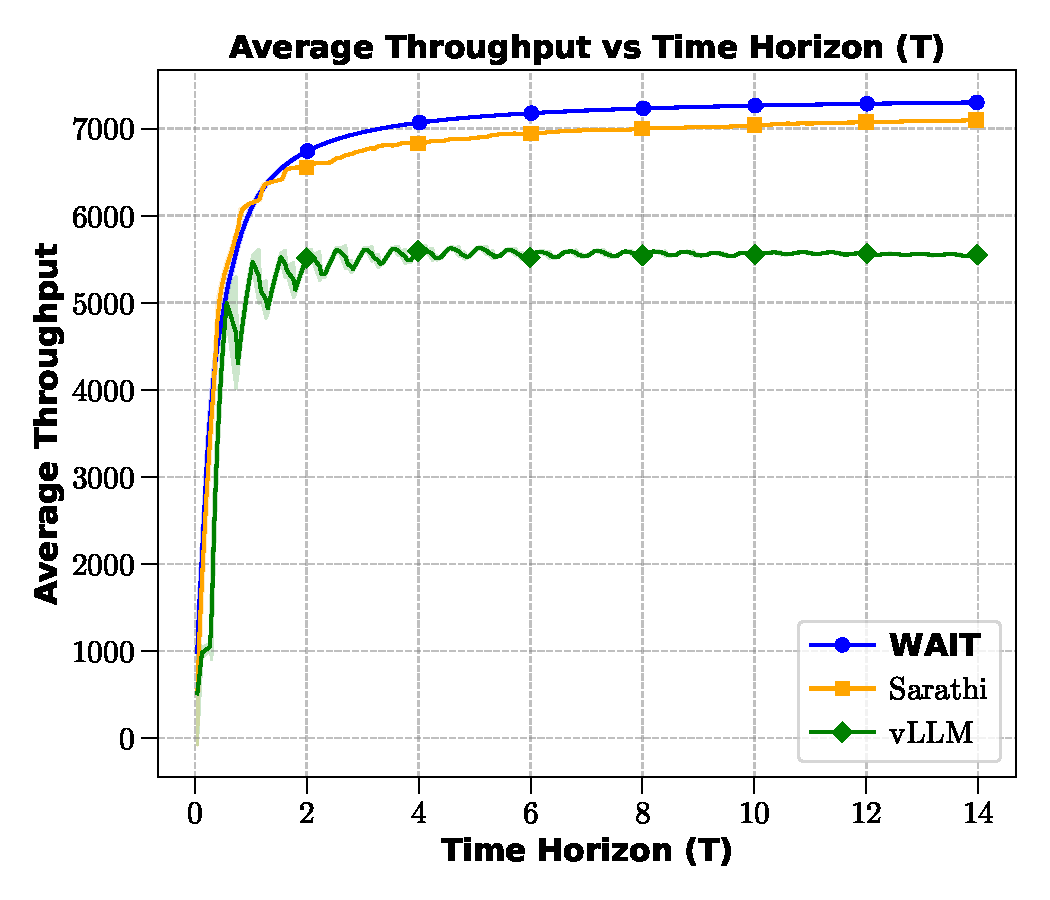
\includegraphics[width=\textwidth]{Experiments_pdf/test9_simulated_short_decode_throughput.pdf}
    \end{minipage}
    \hfill
    \begin{minipage}{0.24\textwidth}
        \centering
        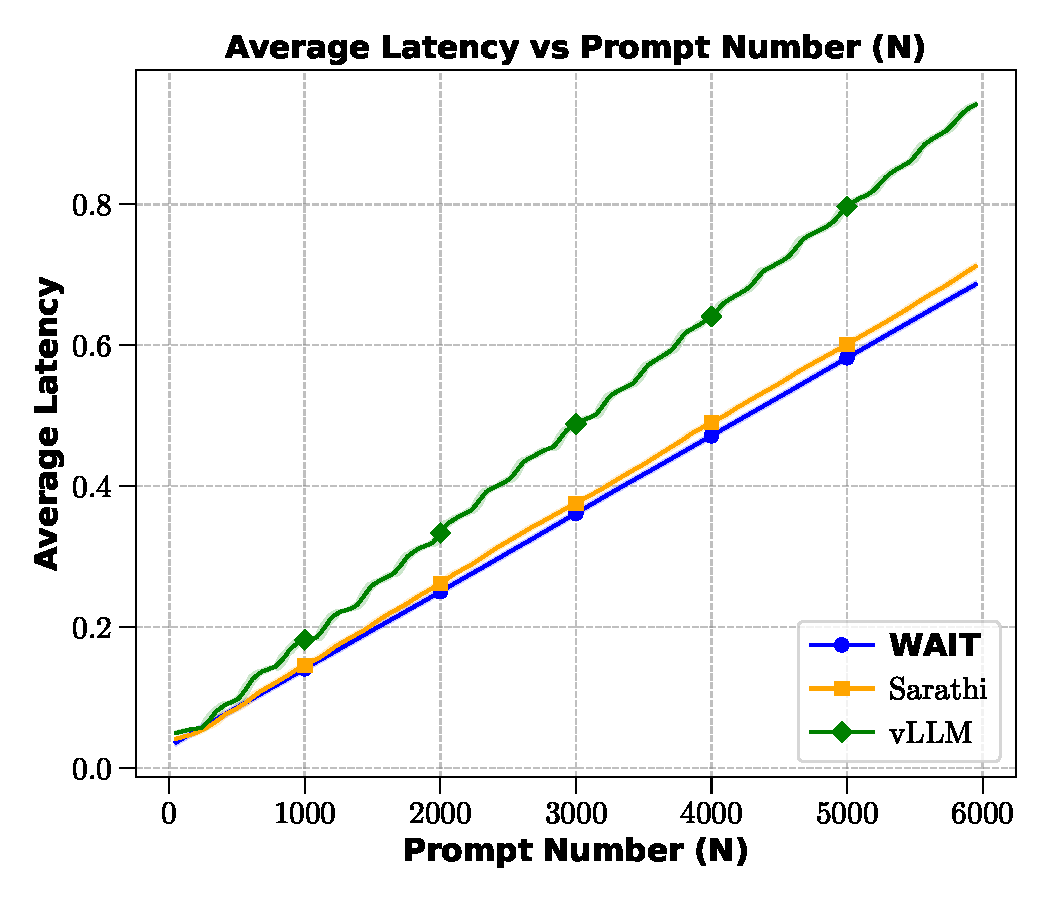
\includegraphics[width=\textwidth]{Experiments_pdf/test9_simulated_short_decode_latency.pdf}
    \end{minipage}
    \hfill
    \begin{minipage}{0.24\textwidth}
        \centering
        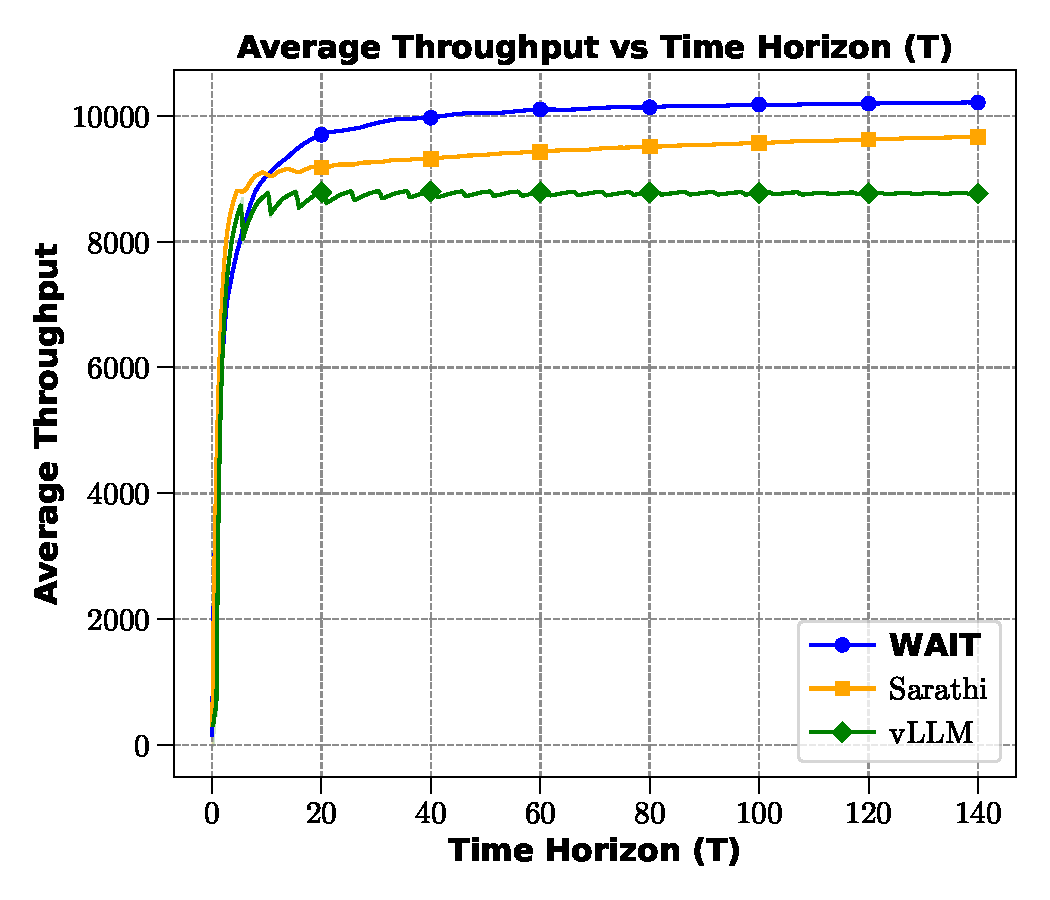
\includegraphics[width=\textwidth]{Experiments_pdf/test13_simulated_short_decode_bs=448_throughput.pdf}
    \end{minipage}
    \hfill
    \begin{minipage}{0.24\textwidth}
        \centering
        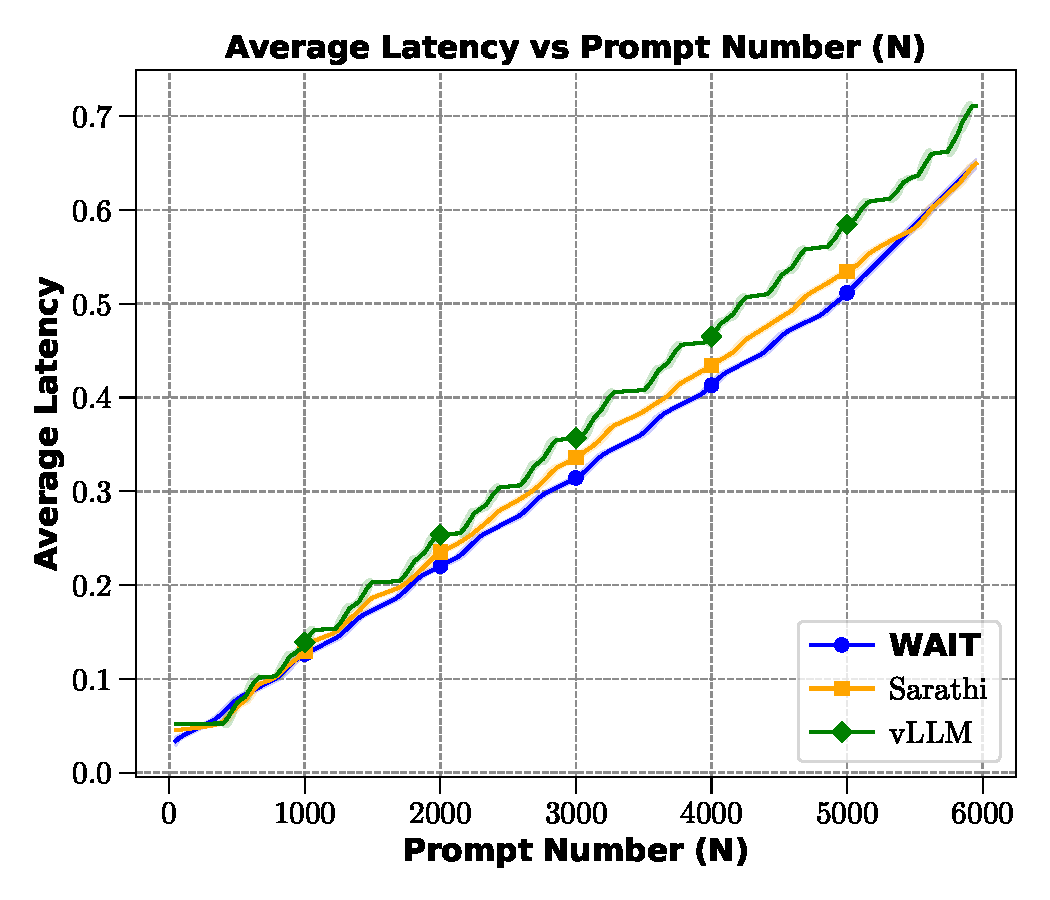
\includegraphics[width=\textwidth]{Experiments_pdf/test13_simulated_short_decode_bs=448_latency.pdf}
    \end{minipage}
    \caption{Multi-type time-series. Left two: low demand; Right two: high demand.}
    \label{fig:comparison WAIT multi}
\end{figure}

\subsection{Nested WAIT (Unknown Output Lengths)}
We test on synthetic data ($m=4$ types, prefill=10, decode=20--160) and LMSYS-Chat-1M \citep{zheng2023lmsys} (50,000 prompts, $L=10$ segments). Figure~\ref{fig:nested_wait_synthetic_lmsys} shows time-series at overloaded rates: Nested WAIT maintains stable throughput while vLLM's declines due to eviction overhead. On-the-fly classification allows short prompts to complete quickly. Figure~\ref{fig:nested_wait_trace} confirms robustness on trace replay: Nested WAIT improves throughput by 15--30\%.
\begin{figure}[htbp]
    \centering
    \begin{minipage}{0.24\textwidth}
        \centering
        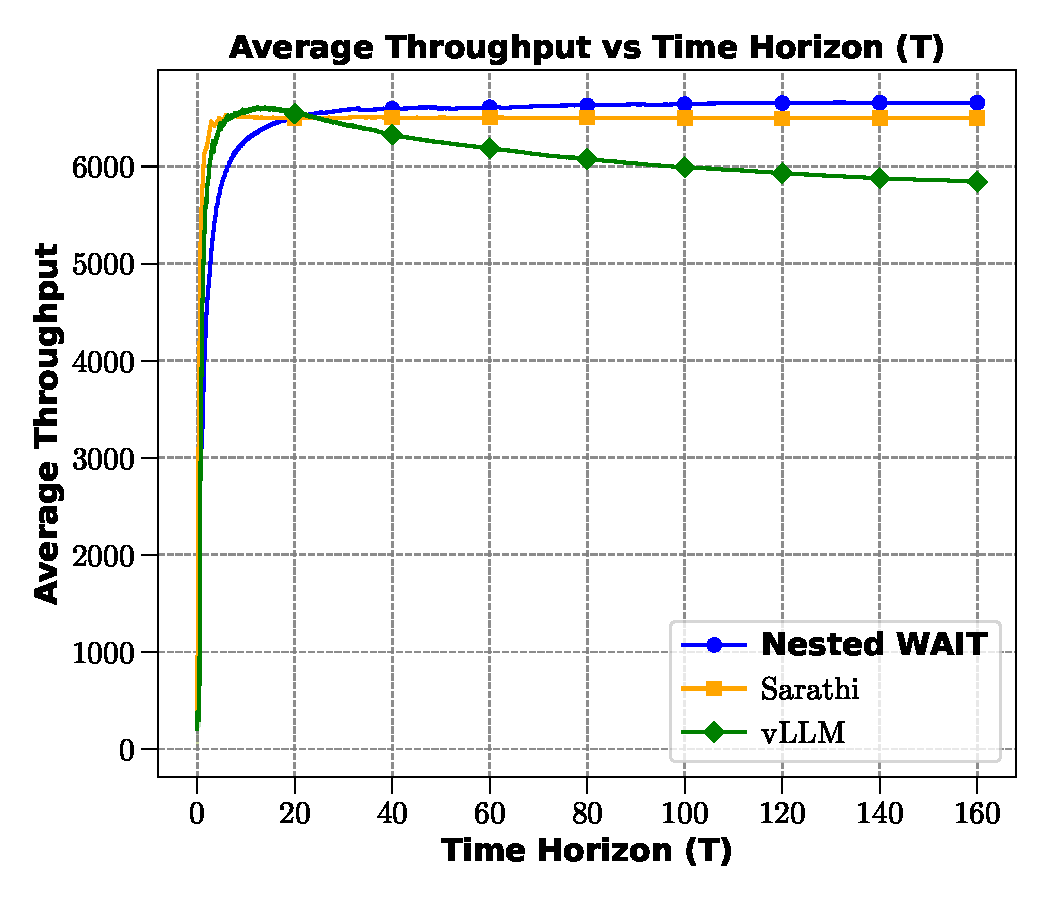
\includegraphics[width=\textwidth]{Experiments_pdf/test30_simulated_short_decode_bs=128_nested_real_not_trace_throughput.pdf}
    \end{minipage}
    \hfill
    \begin{minipage}{0.24\textwidth}
        \centering
        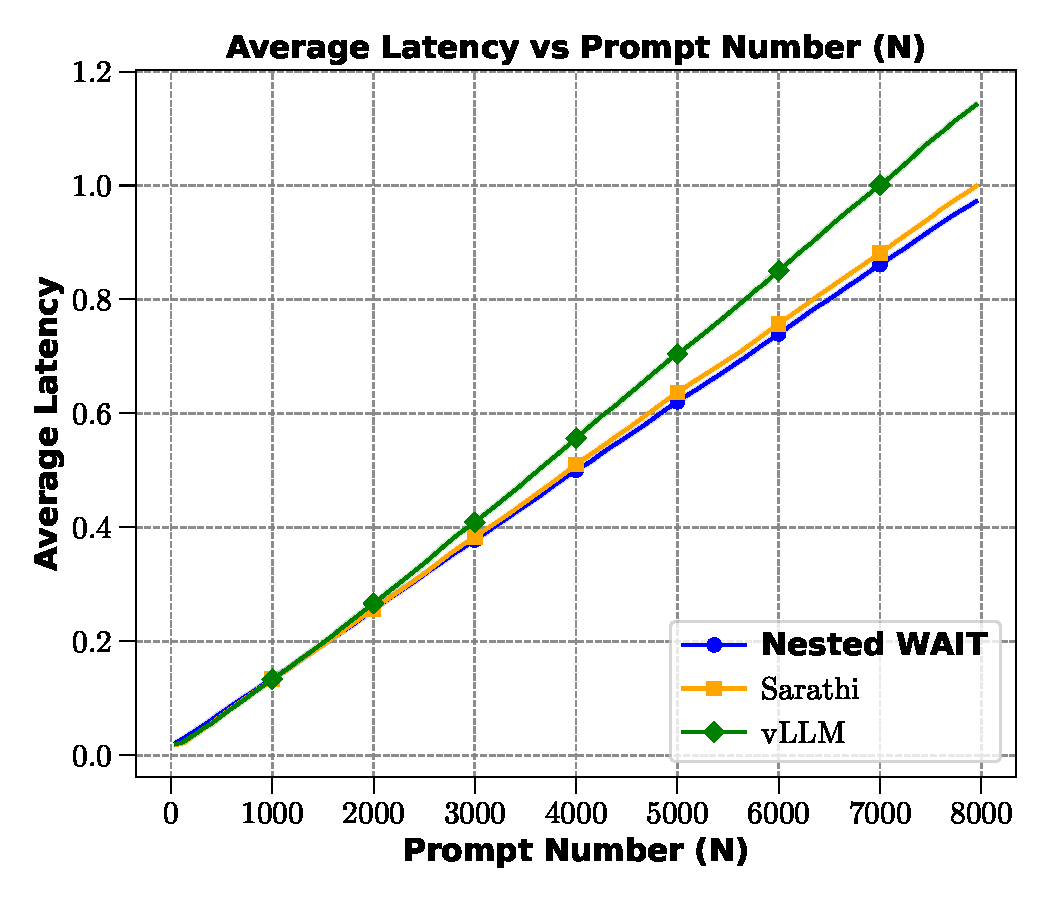
\includegraphics[width=\textwidth]{Experiments_pdf/test30_simulated_short_decode_bs=128_nested_real_not_trace_latency.pdf}
    \end{minipage}
    \hfill
    \begin{minipage}{0.24\textwidth}
        \centering
        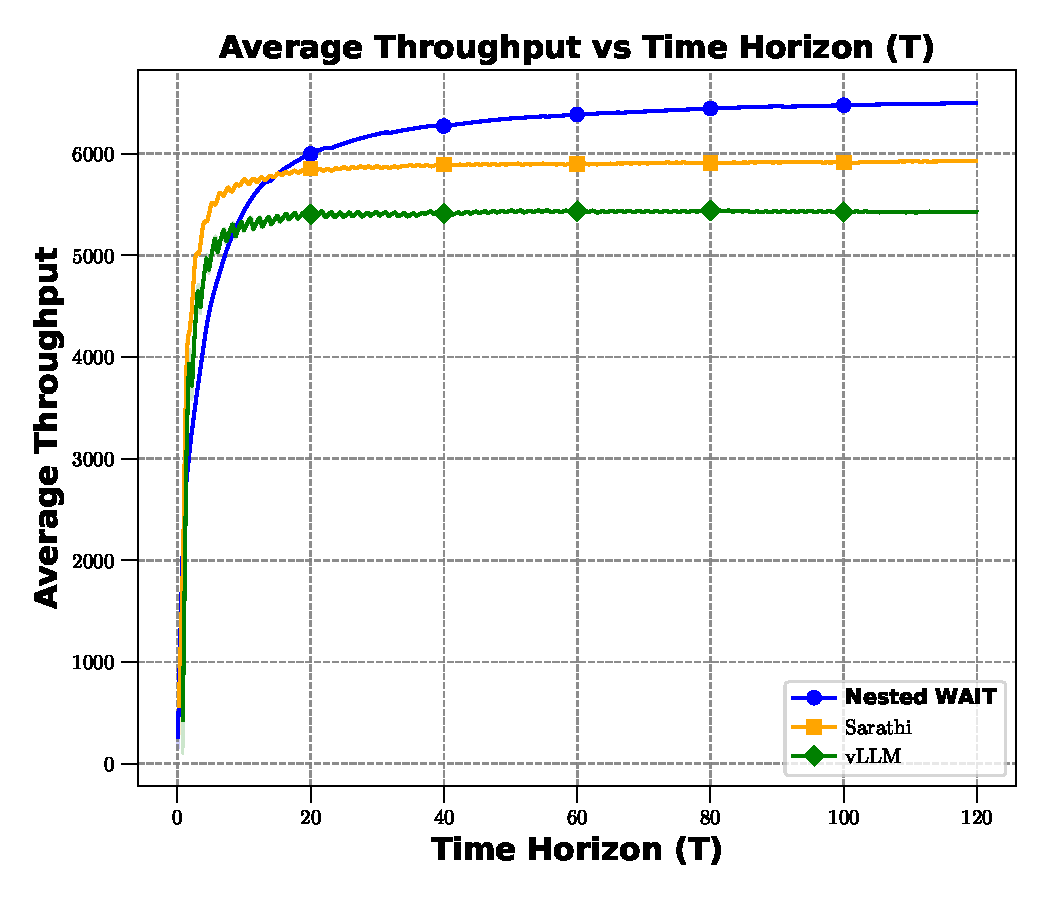
\includegraphics[width=\textwidth]{Experiments_pdf/test32_simulated_short_decode_bs=148_nested_real_not_trace_higher_rate_throughput.pdf}
    \end{minipage}
    \hfill
    \begin{minipage}{0.24\textwidth}
        \centering
        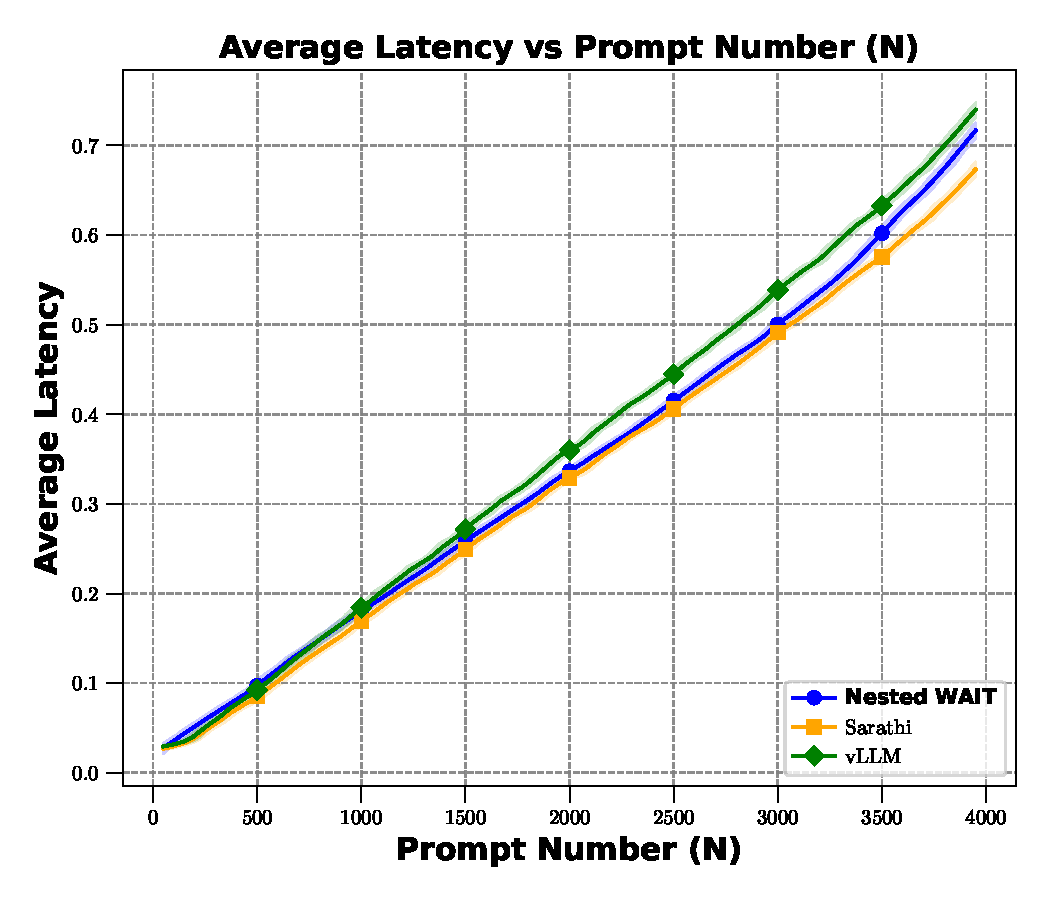
\includegraphics[width=\textwidth]{Experiments_pdf/test32_simulated_short_decode_bs=148_nested_real_not_trace_higher_rate_latency.pdf}
    \end{minipage}
    \caption{Nested WAIT time-series. Left two: synthetic ($m=4$); Right two: LMSYS (QPS=550).}
    \label{fig:nested_wait_synthetic_lmsys}
\end{figure}
\begin{figure}[htbp]
    \centering
    \begin{minipage}{0.45\textwidth}
        \centering
        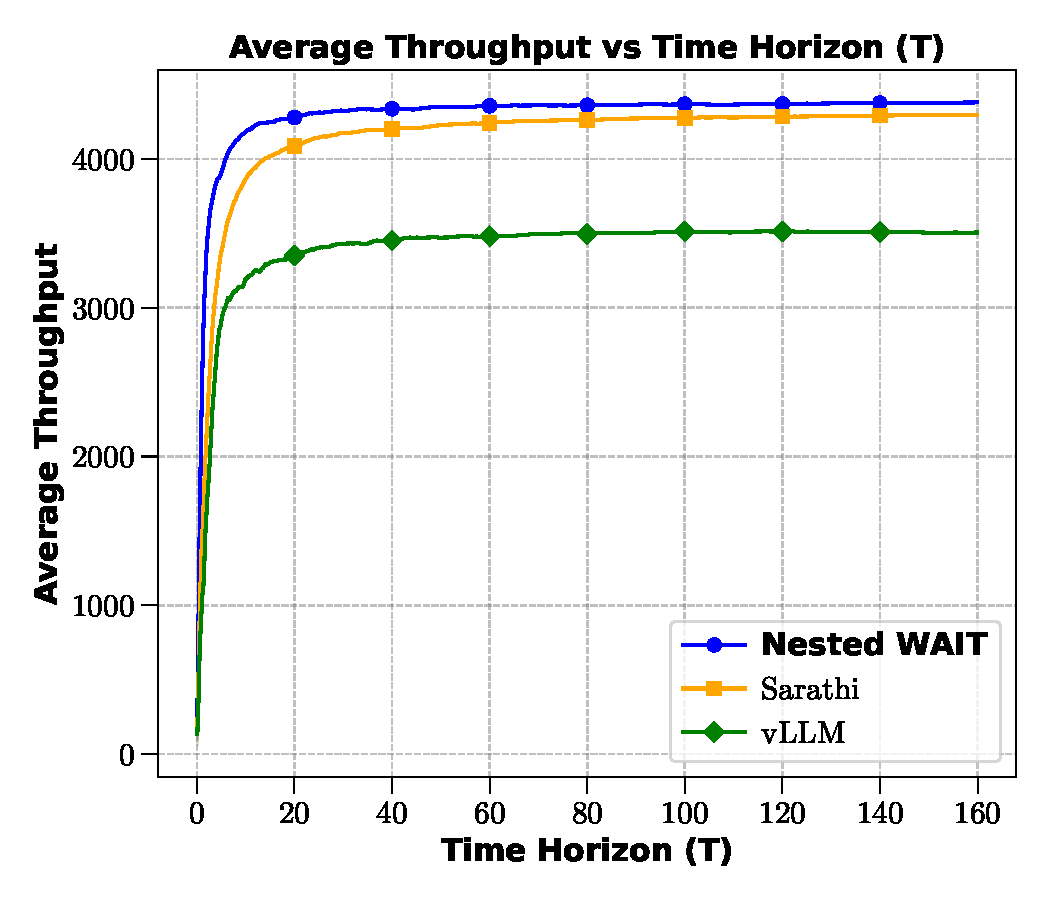
\includegraphics[width=\textwidth]{Experiments_pdf/test36_simulated_short_decode_bs=64_nested_real_TRACE_throughput.pdf}
    \end{minipage}
    \hfill
    \begin{minipage}{0.45\textwidth}
        \centering
        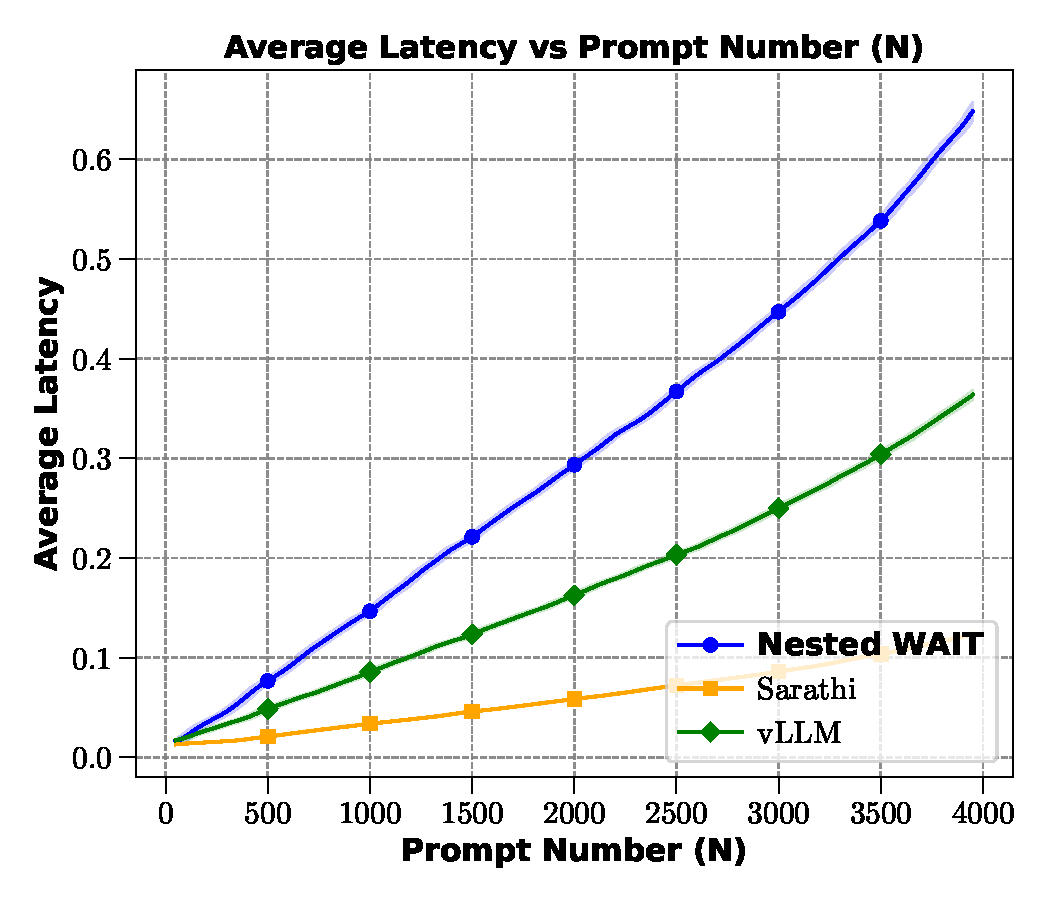
\includegraphics[width=\textwidth]{Experiments_pdf/test36_simulated_short_decode_bs=64_nested_real_TRACE_latency.pdf}
    \end{minipage}
    \caption{Nested WAIT on LMSYS trace replay.}
    \label{fig:nested_wait_trace}
\end{figure}